\documentclass{cubeamer}

\usepackage[french]{babel}
\usepackage{minted}

\usepackage{tcolorbox}
\tcbuselibrary{most,listingsutf8,minted}
\newtcblisting{code}[1]
{
    title=#1,
    hbox,
    sharp corners,
    listing only,
    size=small,
    listing engine=minted,
    minted language=csharp,
    minted options={fontsize=\tiny},
    colback=gray!10
}

\usepackage[T1]{fontenc}
\usepackage{graphicx}

\title{Protection et gestion des licences}
\subtitle{Présentation - Gestion de projet}
\author{Sami Babigeon, Louka Boivin, Kaci Hammoudi, Alexis Osmont}
\date{\today}
\institute[Université de Rouen]{Master Informatique - 1ère année}

\begin{document}

\maketitle
\cutoc

%
%   Exemple de Plan (mail de Karim)
%
%   Présentation rapide du projet (ie. en une phrase/schéma) Revenir sur les engagements pris initialement auprès du client, 
%   détailler le budget projet (adéquation charge/délais) et le périmètre adressé
%   Ces engagements ont-ils été tenus ? Sinon pourquoi ? Quelles ont été les difficultés rencontrées ?
%   Comment avez-vous surmonté ces difficultés ? Quelles solutions ont été mises en œuvre ?
%   Si le projet était à refaire, quels points d’attention garderiez-vous désormais sous contrôle et comment ?
%   Quels acquis faites-vous suite au projet et gestion de votre projet (ie. vos points forts/points de progression) ?
%   Réussite du projet (ie. retours du client) / ouverture / conclusion


% I   Presentation 
% II  Budget \& Périmètre du projet
% III Engagements 
% IV  Difficultés \& Solutions
% V   Améliorations
% VI  Retour d'expèrience
% VII Conclusion

\section{Présentation du projet}

\begin{frame}{Intitulé}
    \centerline{\textbf{Protection et gestion des licences}}
    \medskip
    \emph{Client :}
    \begin{itemize}
        \item M. Ziadi
    \end{itemize}
    \emph{Objectifs :}
    \begin{itemize}
        \item Protection des logiciels du client
        \item Plateforme de gestion pour le client, de demande pour les utilisateurs
        \item Génération et vérification des licences
    \end{itemize}
\end{frame}

\begin{frame}{Présentation Général}
    \begin{figure}
        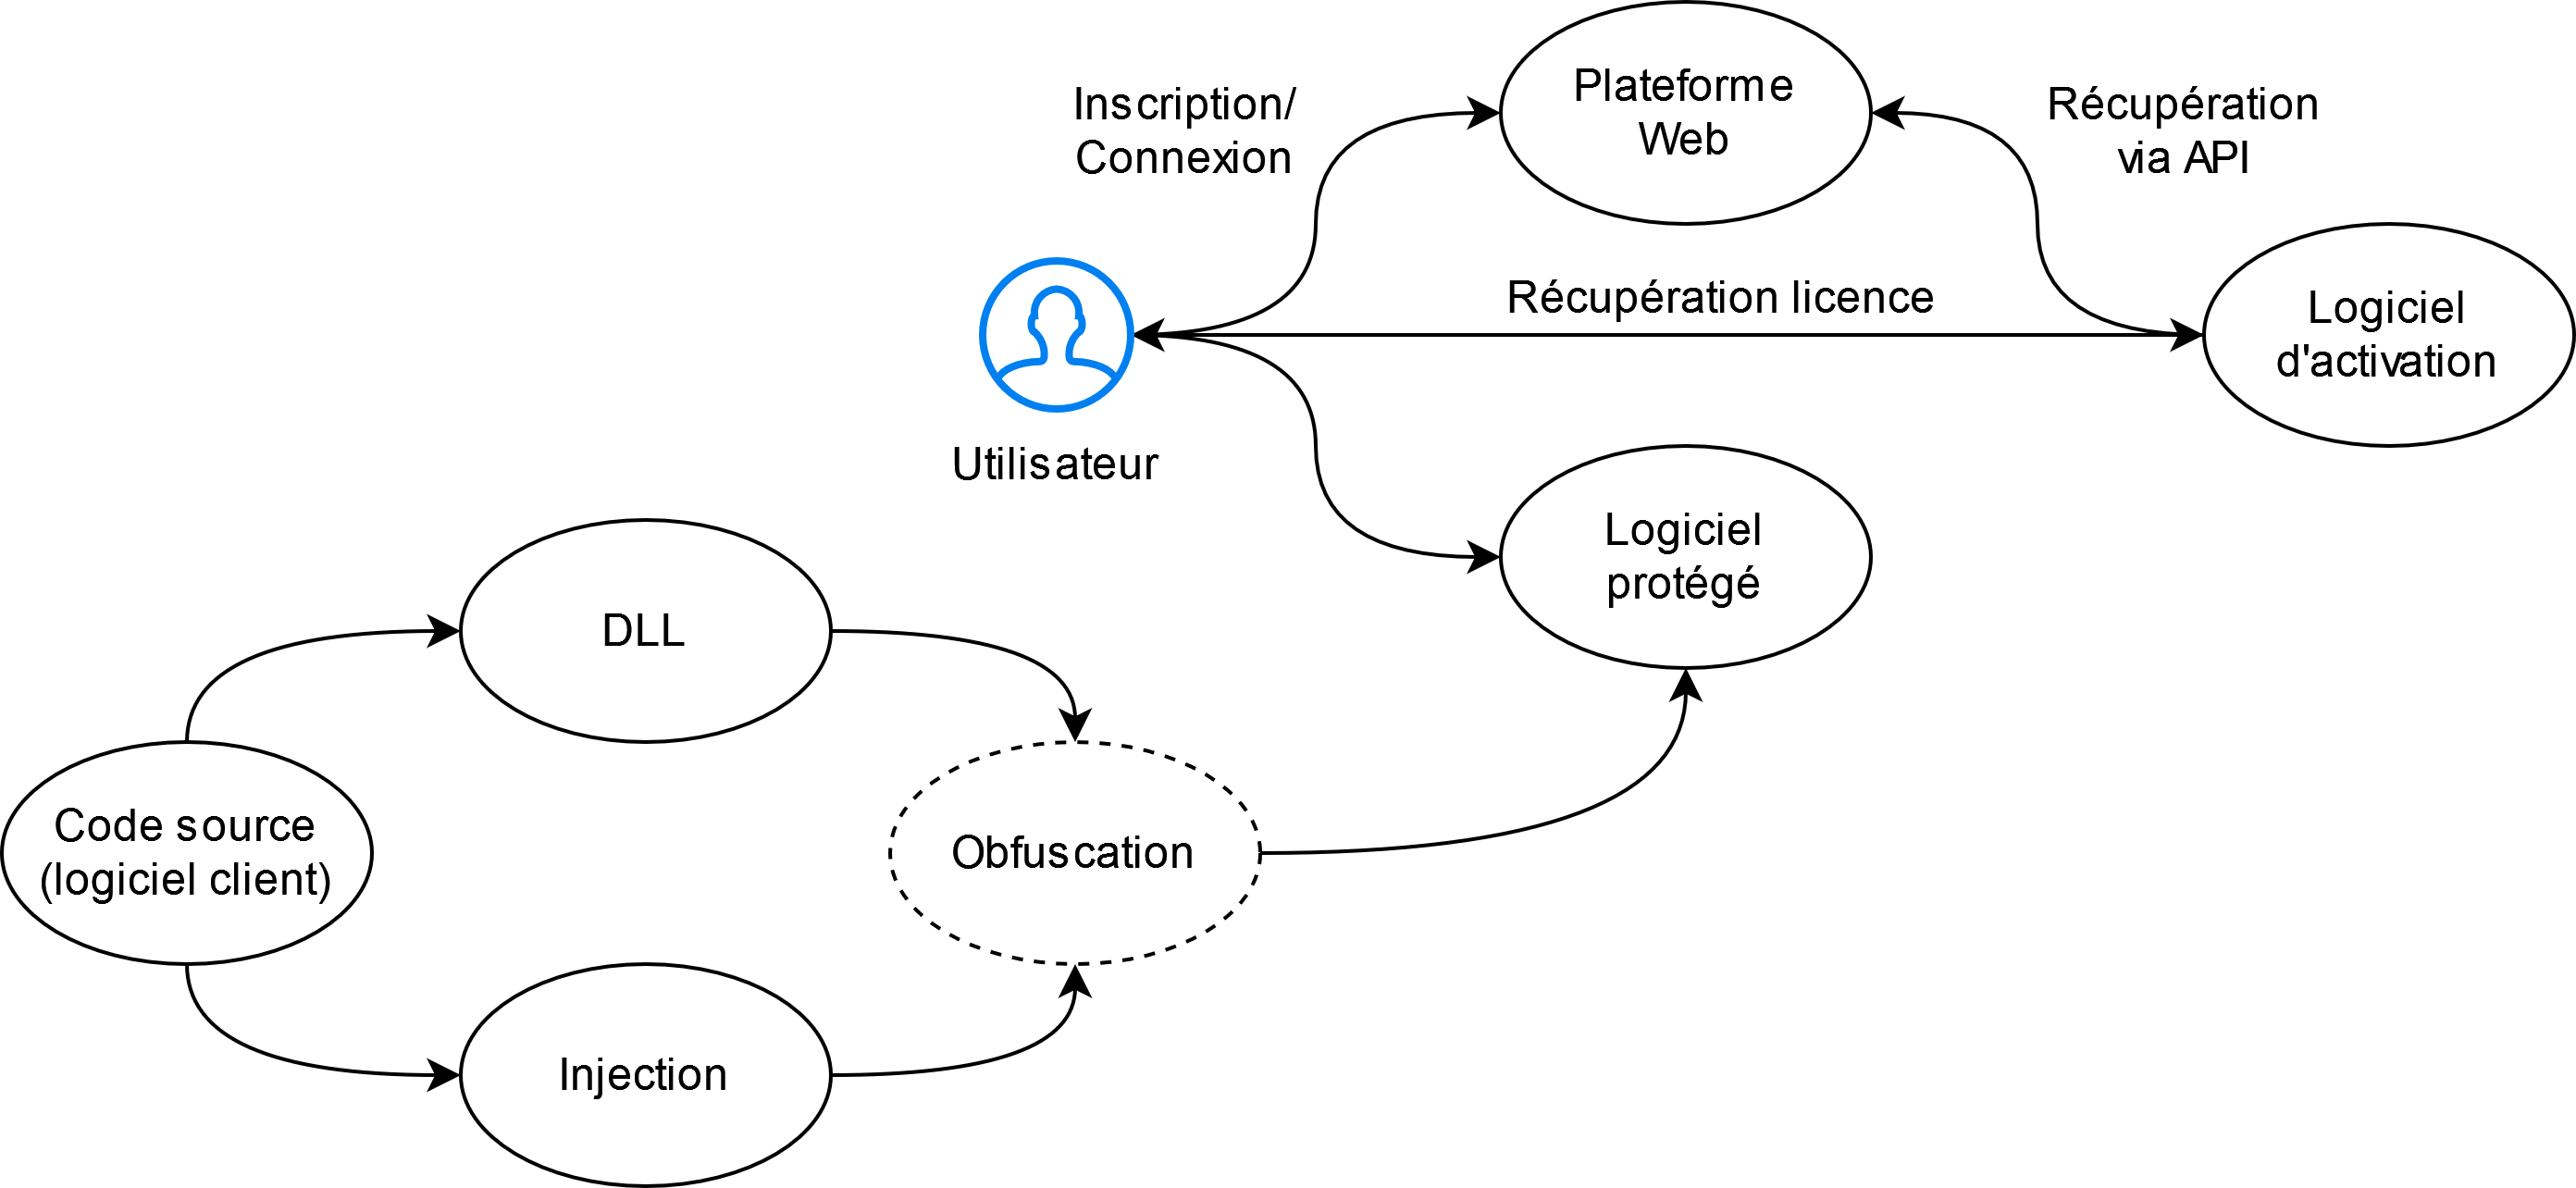
\includegraphics[scale=0.7]{img/general.png}
    \end{figure}
\end{frame}

\section{Engagements}

\begin{frame}{Budget initial}
    \begin{itemize}
        \item 200 heures estimées
        \item 5 membres dans l'équipe
        \item 2 machines virtuelles
      \end{itemize}
 %   \begin{figure}
 %       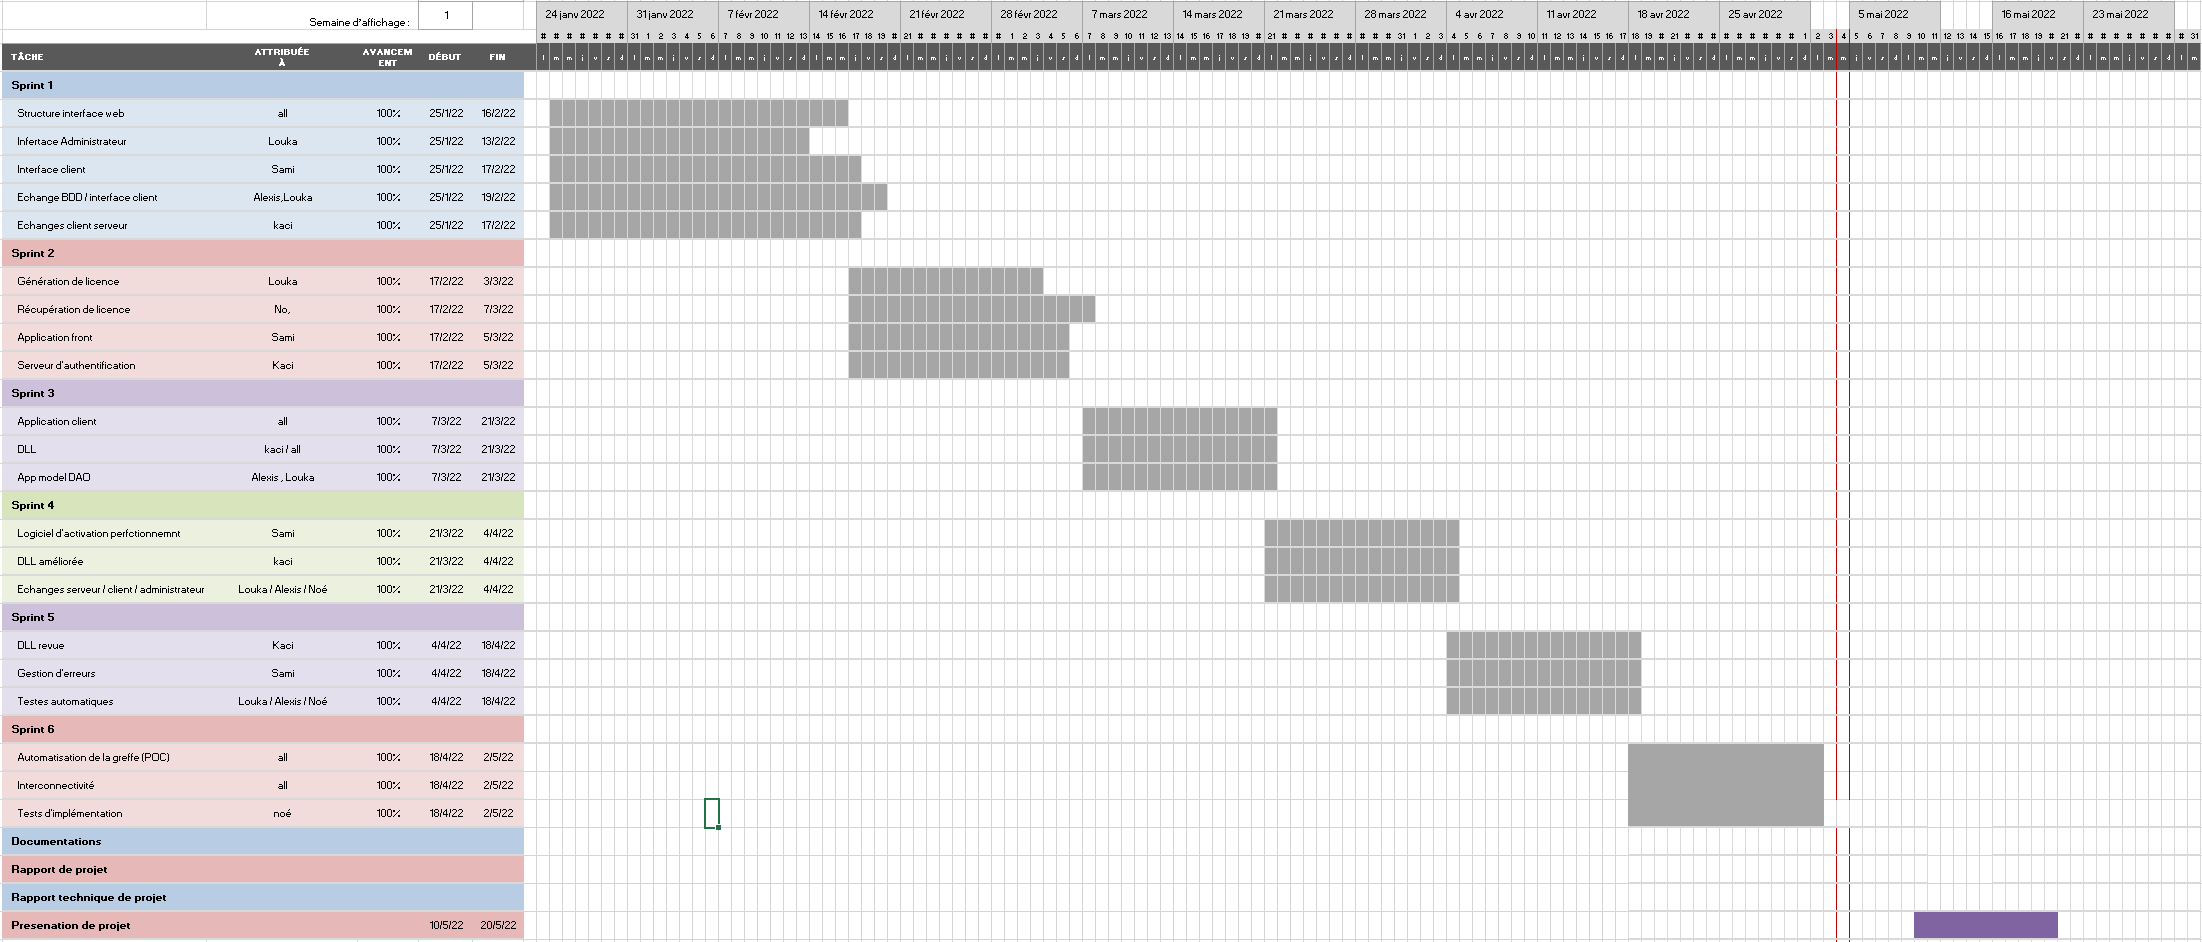
\includegraphics[scale=0.24]{img/Gantt.png}
 %   \end{figure}
\end{frame}

\begin{frame}{Engagements}
    \begin{itemize}
        \item Système de vérification de licence fonctionnel
        \begin{itemize}
        \item Bibliothèque de fonctions
        \item Plateforme web
        \item Logiciel d'activation
        \item Détection de fraude
        \item Obfuscation
        \item Injection de code / greffe 
        \end{itemize}
        \item Documentation
    \end{itemize}
\end{frame}

\section*{Engagements tenus}

\subsection{Présentation - Front}

\begin{frame}{Front - Plateforme web}
    \begin{columns}

        \begin{column}{.25\textwidth}
            Une interface web            
            \begin{itemize}
                \item Sécurisé \\{\scriptsize{(webfilter, \verb:Bcrypt:)}} 
                \item Ergonomique {\scriptsize({utilisation de \verb:Bootstrap:)}}
            \end{itemize}
        \end{column}

        \begin{column}{.75\textwidth}
            \begin{figure}
                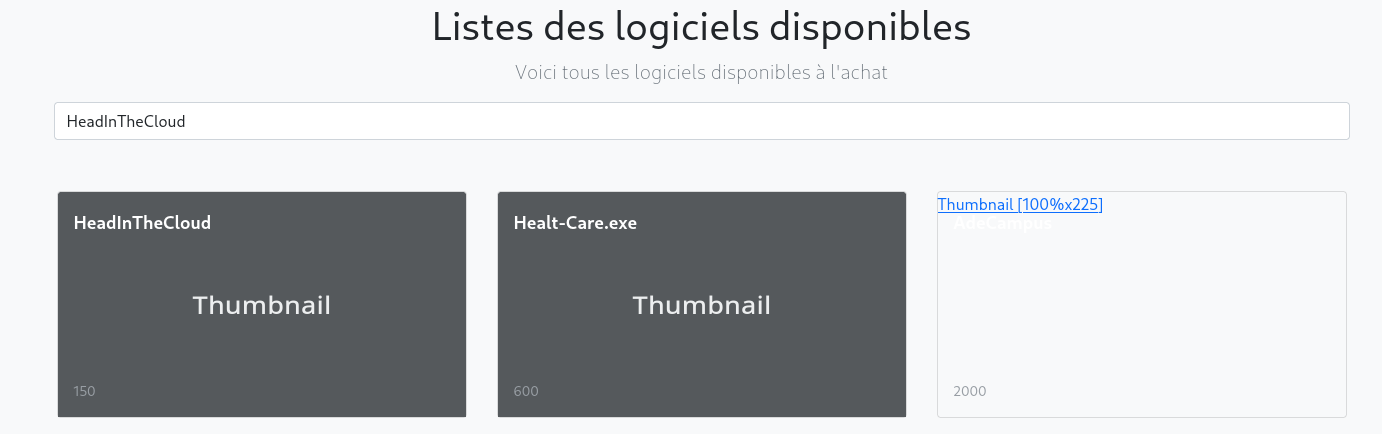
\includegraphics[scale=0.27]{img/web1.png}
            \end{figure}  
        \end{column} 

    \end{columns}

\end{frame}

\begin{frame}{Front - Plateforme web}
    \begin{columns}
        \begin{column}{.70\textwidth}
            \begin{figure}
                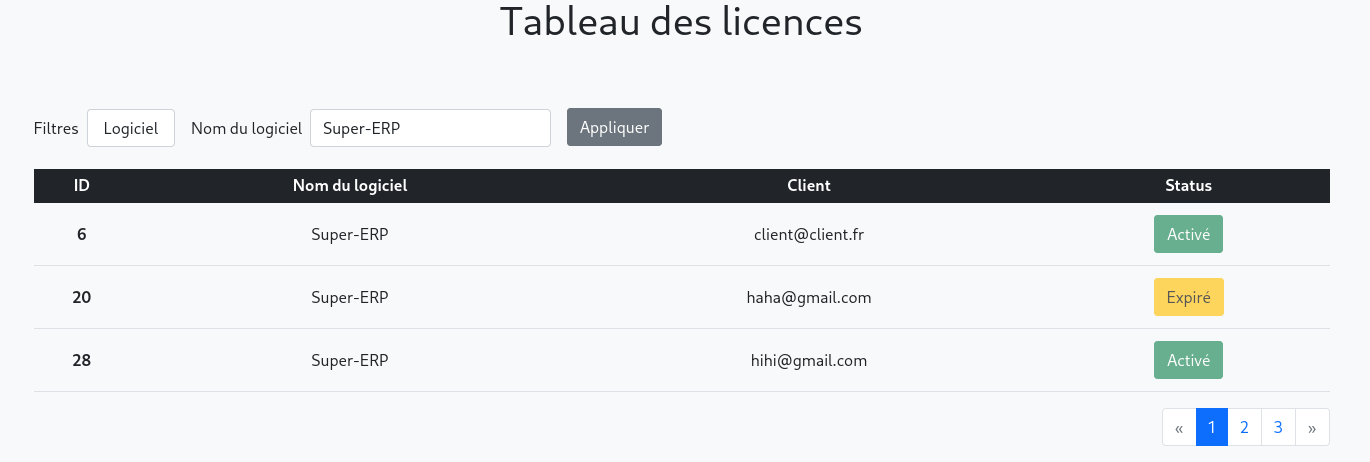
\includegraphics[scale=0.27]{img/web3.png}
            \end{figure}  
        \end{column}
 
        \begin{column}{.3\textwidth}
            permet à un client:            
            \begin{itemize}
                \item Acheter une licence pour un logiciel  
                \item Consulter la liste de ces logiciels 
            \end{itemize}
        \end{column}

    \end{columns}
\end{frame}

\begin{frame}{Front - Plateforme web}
        \begin{columns}

        \begin{column}{.25\textwidth}
            permet à l'administrateur:
            \begin{itemize}
                \item De valider ou d'invalider une licence
                \item Ajouter et de lister les logiciels
            \end{itemize} 
        \end{column}

        \begin{column}{.75\textwidth}
            \begin{figure}
                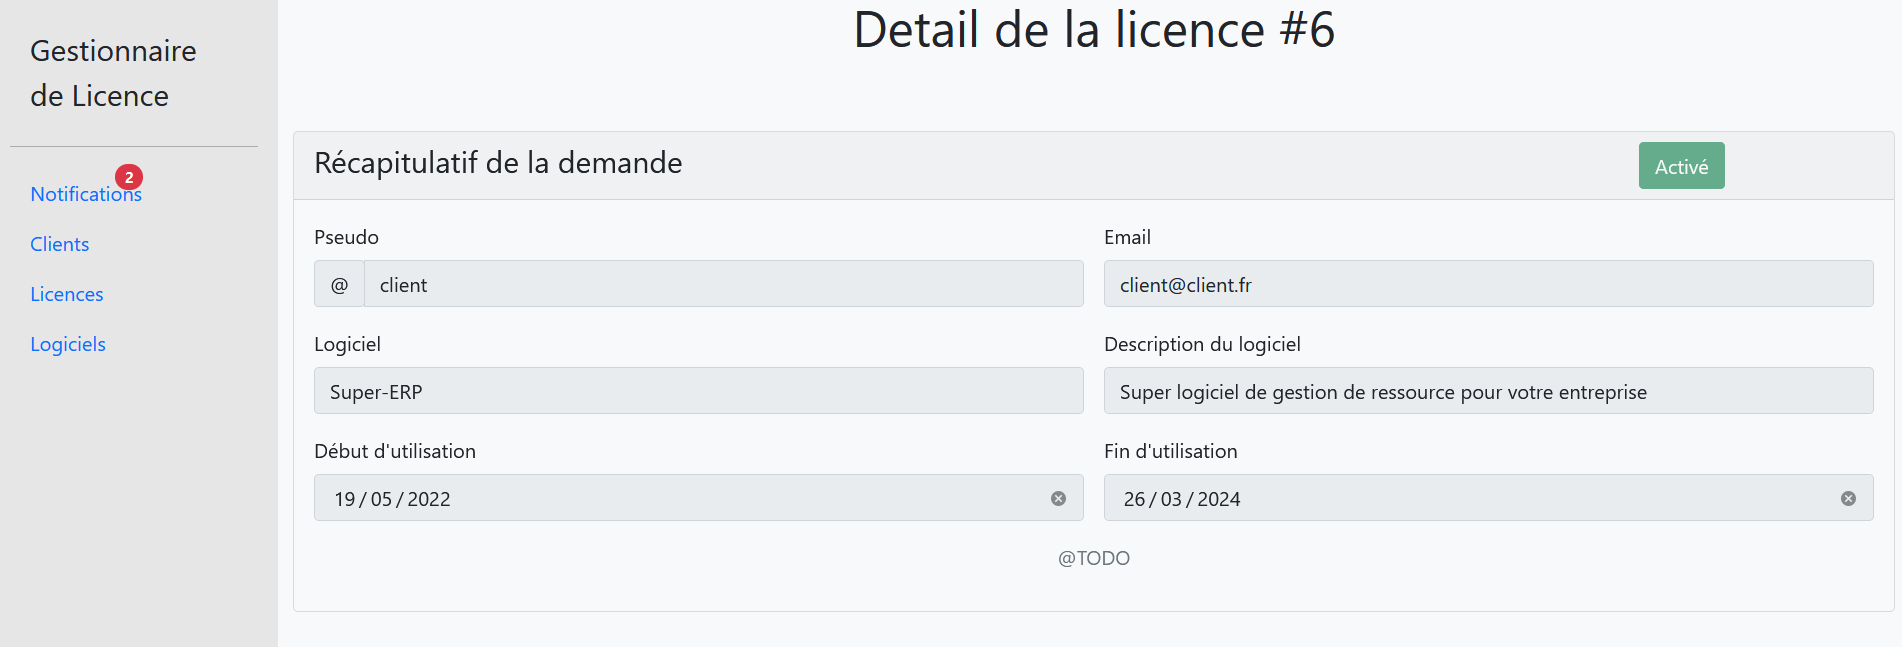
\includegraphics[scale=0.27]{img/web2.png}
            \end{figure}  
        \end{column} 

    \end{columns}       
\end{frame}

\begin{frame}{Front - Logiciel d'activation}
    \begin{columns}

        \begin{column}{.5\textwidth}
            Permet à un client de:
            \begin{itemize}
                \item Envoyer l'identifiant hardware au serveur 
                \item Récuperer une licence pour un logiciel (via API)
            \end{itemize}
        \end{column}

        \begin{column}{.5\textwidth}
            \begin{figure}
                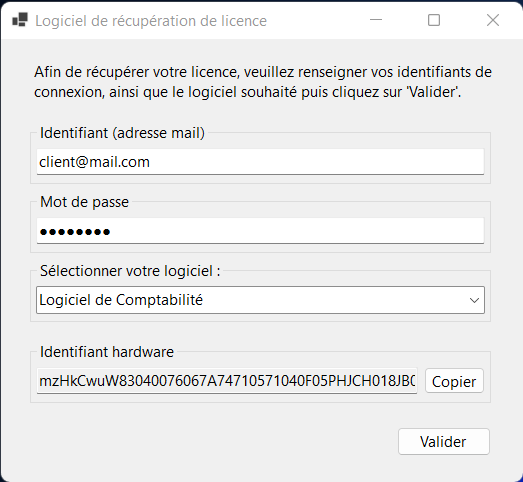
\includegraphics[scale=0.5]{img/activation-soft.png}
            \end{figure}  
        \end{column} 

    \end{columns}
\end{frame}

\subsection{Présentation - Back}

\begin{frame}{Back - Génération Licence}
    \begin{columns}
    \begin{column}{0.4\textwidth}
        Signature :
        \begin{itemize}
            \item ECDSA
            \item \verb:secp256k1:
            \item \verb:java.security.Signature:
        \end{itemize}
    \end{column}
    \begin{column}{0.6\textwidth}  
        \vspace{-1cm} 
        \begin{figure}
            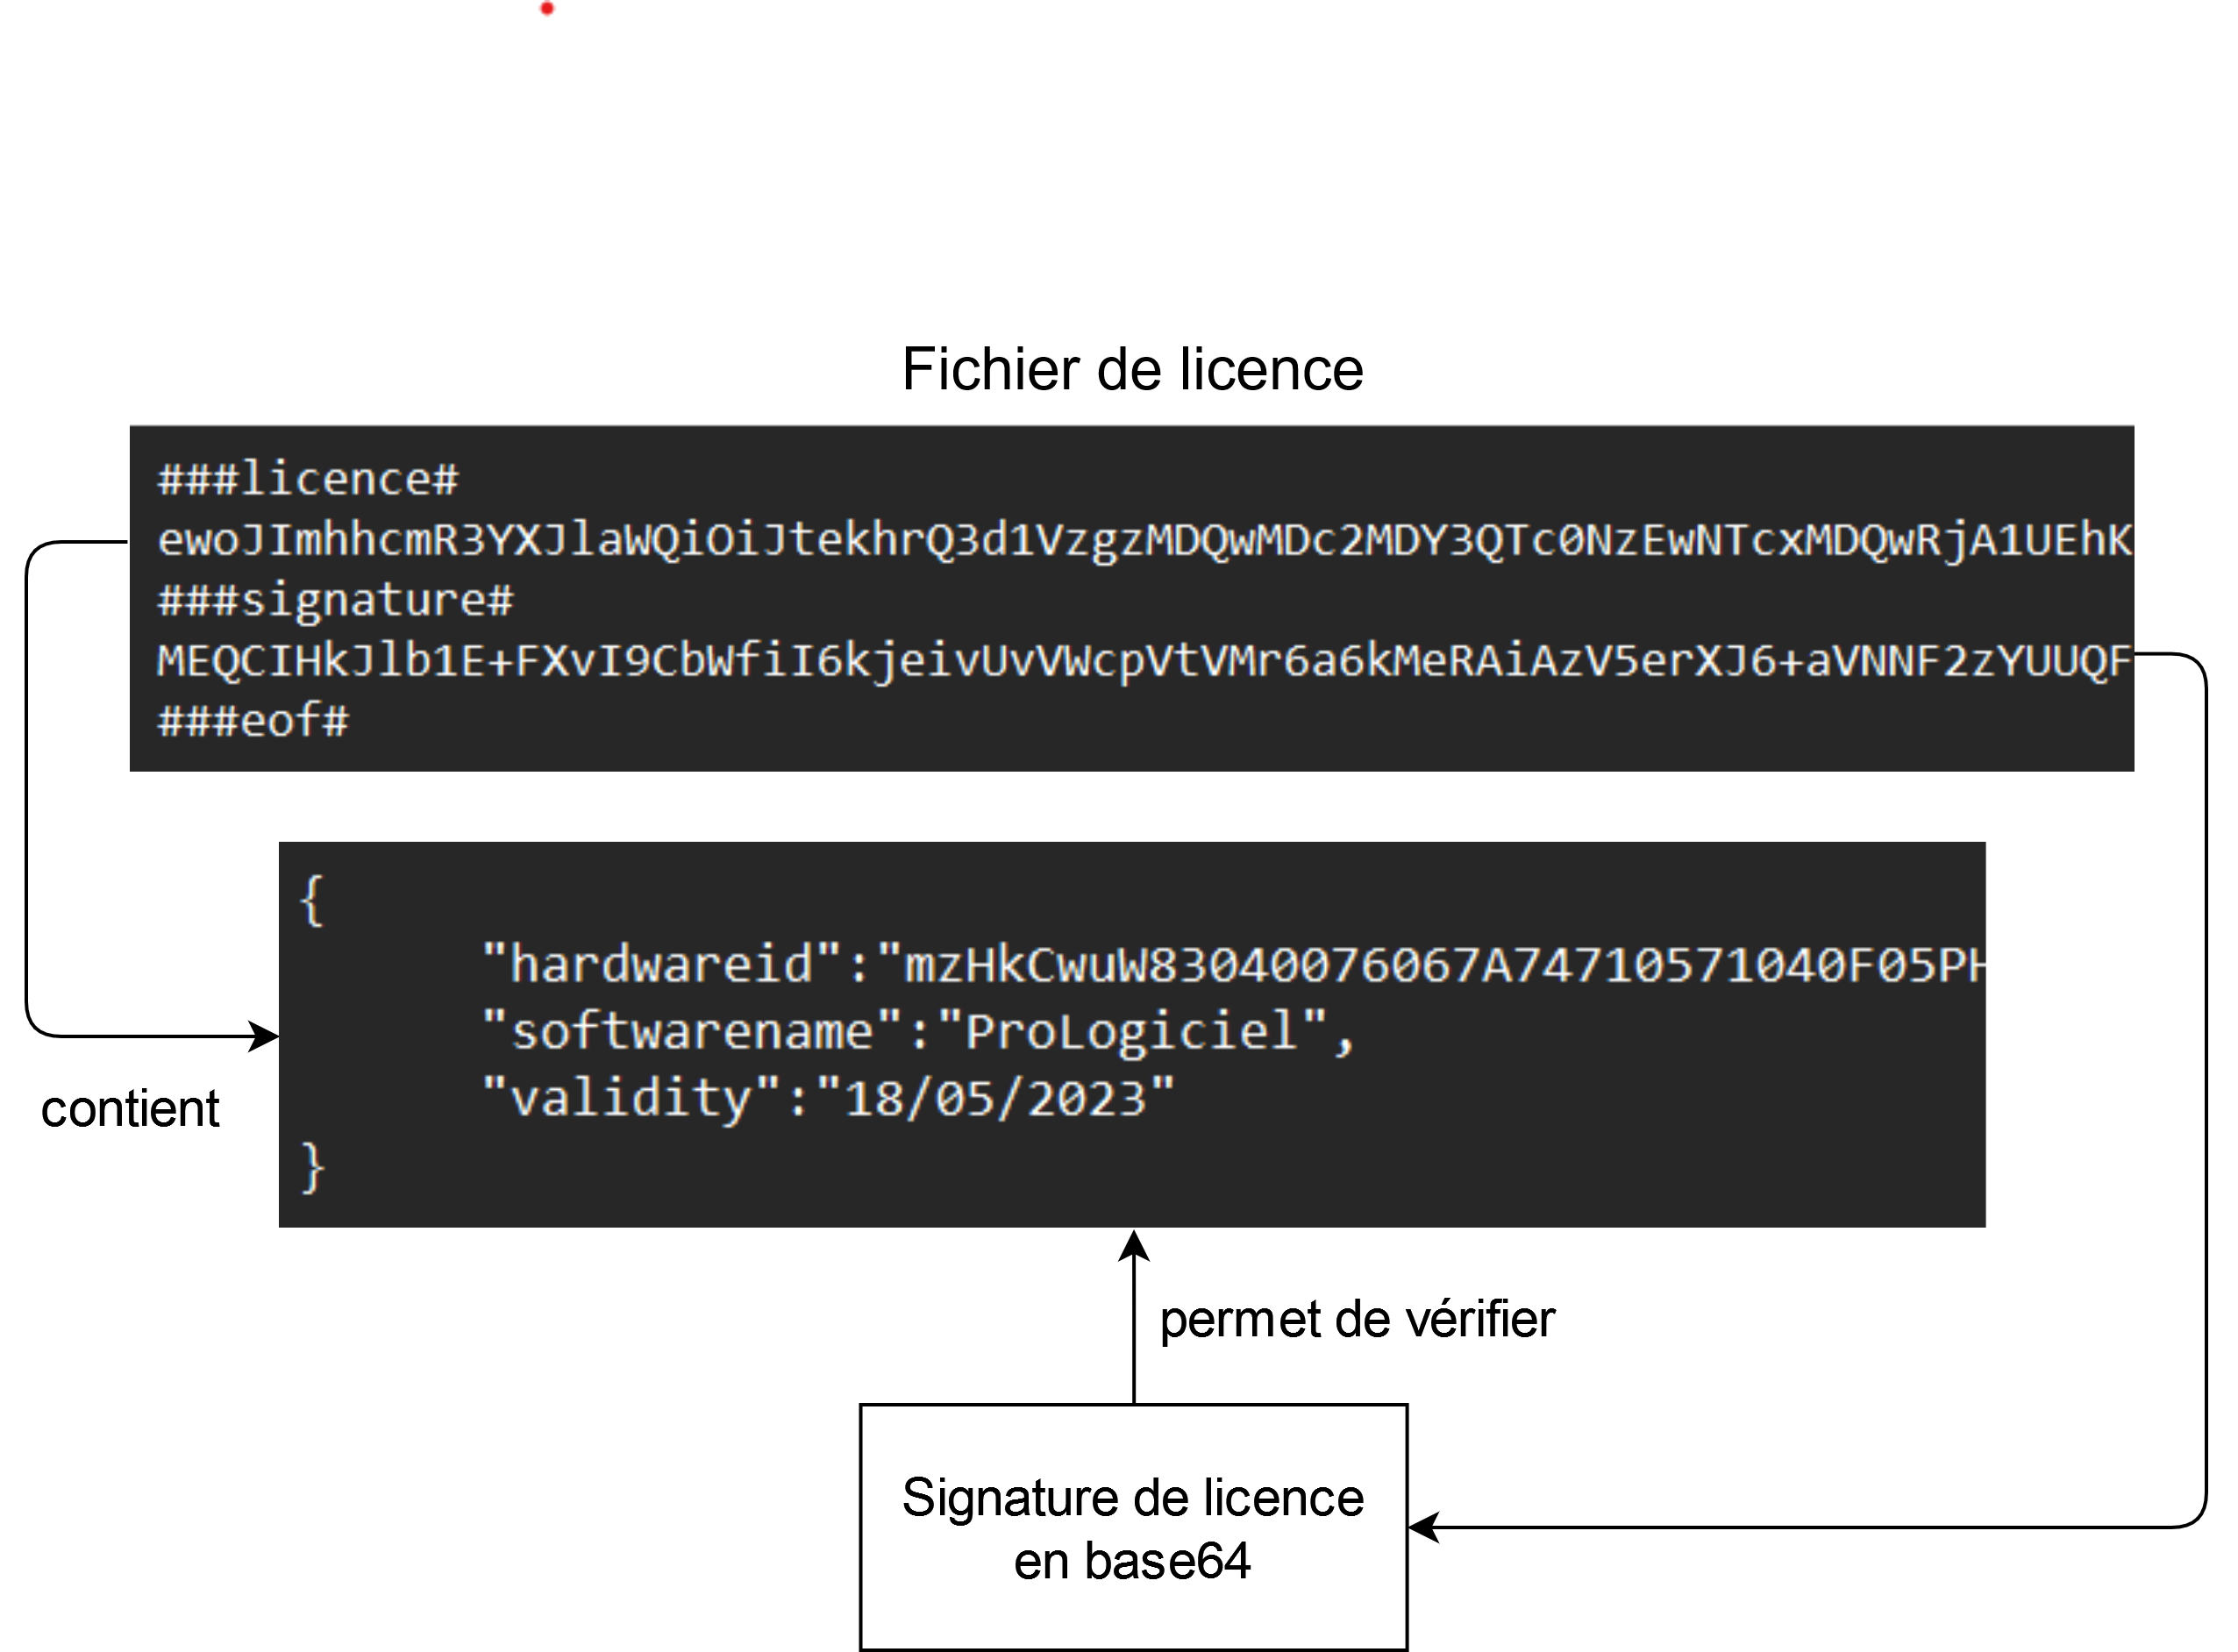
\includegraphics[scale=0.5]{img/licence.png}
        \end{figure}
    \end{column}
    \end{columns}
\end{frame}

\begin{frame}[fragile]{Back - DLL}
    \begin{columns}

        \begin{column}{.28\textwidth}
            \begin{figure}
                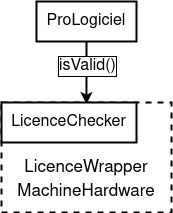
\includegraphics[scale=2.5]{img/Prologiciel.png}
            \end{figure}
        \end{column}

        \begin{column}{.72\textwidth}
\begin{code}{}
private const string SOFTWARE_NAME = <Nom du logiciel>;
private const string LICENCE_FILE_PATH = <Chemin vers le fichier de licence>;

static public void Main()
{
    // Création d'une instance de LicenceChecker.
    LicenceChecker licenceChecker = new LicenceChecker(LICENCE_FILE_PATH, SOFTWARE_NAME);
    // Ajout des paramètres de l'identifiant hardware.
    licenceChecker.setHardwareHashComposent(true, true, true, true, true);
    // Test de la licence.
    if (!licenceChecker.isValid())
    {
        Console.WriteLine("Integrité ou Validité de la licence non valide.\n"
            + "Refus de lancer le logiciel.\n");
        return;
    }
    // La licence est valide. Le logiciel peut se lancer.
    Console.WriteLine("ProLogiciel peut se lancer à présent.\n"
        + "Hello World !\n");
    return;
}
\end{code}
        \end{column}
    \end{columns}
\end{frame}

\begin{frame}[fragile]{Back - DLL}
    \begin{columns}

        \begin{column}{.28\textwidth}
            \begin{figure}
                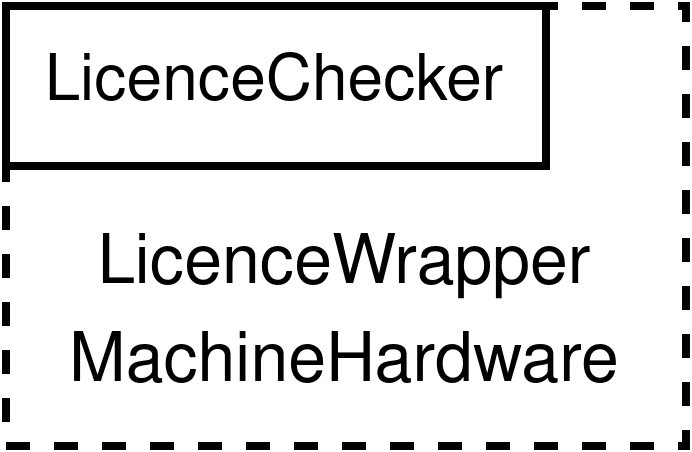
\includegraphics[scale=0.5]{img/dllschemamini.png}
            \end{figure}
            La \verb:DLL: permet de:
            \begin{itemize}
                \item Vérifier la validité 
                \item Vérifier l'integrité
                \item Invalider la licence
            \end{itemize}
        \end{column}

        \begin{column}{.72\textwidth}
\begin{code}{}
public bool isValid()
{
    return checkIntegrity() && checkValidity() && antiCheatTest();
}

public bool checkIntegrity()
{
    return checkSignature();
}

public bool checkValidity()
{
    return checkHardwareHash() && checkExpirationDate() && checkName();
}

public void invalidateLicence()
{
    RegistryKey key;
    key = Registry.CurrentUser.CreateSubKey("ProLicenceMachineHardware");
    key.DeleteValue("anticheating_CODE");
    Console.WriteLine("\nLa licence a été invalidée.\n");
}
\end{code}
        \end{column}
    \end{columns}
\end{frame}

\begin{frame}[fragile]{Back - Detection de fraude}
    \begin{columns}
        \hspace{-1cm} 
        \begin{column}{.4\textwidth}

\begin{code}{}
private static string assureAntiCheating()
{
    RegistryKey key;
    key = Registry.CurrentUser.CreateSubKey("ProLicenceMachineHardware");
    String? anticheatcode = key.GetValue("anticheating_CODE")?.ToString();
    if (anticheatcode == null)
    {
        // Génération d'une clé aléatoire
        Random random = new Random();
        string newcode = "";
        for (var i = 0; i < ANTICHEAT_CODE_LEN; i++)
        {
            int r = random.Next(ALPHABET.Length);
            newcode += ALPHABET[r];
        }
        key.SetValue("anticheating_CODE", newcode);
        key.Close();
        return newcode;
    }
    key.Close();
    return anticheatcode;
}
\end{code}            
        \end{column}

        \begin{column}{.5\textwidth}
            \begin{itemize}\raggedleft
                \item Signature de licence
                \item Détection de date
                \item Machine HardwareId
            \end{itemize}
\begin{code}{}
public static bool SOtimeChange()
{
    bool time = false;
    string oldTime = "S-1-1-22";    

    EventLog log = new EventLog("Security");
    var entries = log.Entries.Cast<EventLogEntry>()
        .Where(x => x.TimeWritten >= DateTime.Now.AddHours(-72))
        .Select(x => new {x.InstanceId,x.ReplacementStrings}).ToList();

            foreach (var entrie in entries)
            {
                if (entrie.InstanceId == 4616)
                {
                    time = !entrie.ReplacementStrings[0].Contains(oldTime);
                }
            }
    return time;
}
\end{code}                    
        \end{column}

    \end{columns}
\end{frame}

\section{Difficultés rencontrées \& Solutions proposées}

\begin{frame}{Difficultés rencontrées}
    \begin{itemize}
        \item Difficultés Techniques 
              \begin{itemize}
                \item Injection de code
                \item Détection de fraude
                \item Obfuscation
                \item Problème de Réseau
              \end{itemize}
        \item Difficultés Humaines
              \begin{itemize}
                \item Abandon d'un membre du groupe
                \item Communication
                \item Cerner les attentes du client
              \end{itemize}
    \end{itemize}
\end{frame}

\begin{frame}{Solutions proposées}
    \begin{itemize}
        \item Mise en place de protections simple
        \item Configuration réseau statique
        \item Revue du périmètre du projet
        \item Ré-organisation des tâches
        \item Réunion regulière \& utilisation des outils comme \verb:trello:
    \end{itemize}
\end{frame}

\section{Améliorations}

\begin{frame}{Améliorations}
    \begin{columns}
        \begin{column}{0.5\textwidth}
            En gestion de projet :
            \begin{itemize}
                \item Revoir les priorités et l'estimation
                \item Plus communiquer (entre nous, avec le client)
                \item Anticiper les risques
            \end{itemize}
        \end{column}
        
        \begin{column}{0.5\textwidth}
            Techniques :
            \begin{itemize}
                \item Poursuivre la greffe de code
                \item Utilisation de framework pour la partie développement
            \end{itemize}
        \end{column}
    \end{columns}
\end{frame}

\section{Retour d'expérience}

\begin{frame}{Retour d'expérience}
    \begin{itemize}
        \item Compétences techniques 
            \begin{itemize}
                \item Programmation Windows 
                \item Connaissances sur les techniques d'injection de code
                \item Mise en place d'un système composé de plusieurs élements
                \item Mise en pratique d'outils cryptographiques
            \end{itemize}
        \item Compétences en Gestion de projets
             \begin{itemize}
                \item Amélioration de nos compétences en gestion de projets \\
                  notamment sur les outils (\verb:git:, \verb:trello:)
                \item Communication \& Organisation
                \item Gestion d'un client
            \end{itemize}           
    \end{itemize}
\end{frame}

\section{Conclusion}

%\begin{frame}{Conclusion}
%    \begin{itemize}
%        \item Première approche de la gestion de projet 
%        \item Client satisfait dans l'ensemble
%        \item Engagements tenus
%    \end{itemize}
%\end{frame}

%\section*{Démonstration}

% Q&A
\begin{frame}[standout]
    \Huge\textsc{Merci de votre écoute}
    \vfill
    \LARGE\textsc{Questions ?}
\end{frame}

\end{document}

